\documentclass[12pt,fleqn]{article}
\usepackage{
  amsmath,
  hyperref,
  booktabs,
  geometry,
  graphicx,
  microtype,
  parskip,
}
\usepackage[shortlabels]{enumitem}

\geometry{margin=3cm}

% equation line spacing
\setlength{\jot}{0.5cm}

% meta data
\newcommand{\chapter}{Chapter 1\--3}
\newcommand{\authorname}{Amo DelBello}
\newcommand{\classdescription}{MATH 1350-D2}
\newcommand{\classname}{Introduction to Statistics, Fall 2022}
\newcommand{\assignment}{\chapter\ Take Home Exam}

\newcommand{\problem}[1]{\vspace{5ex}\section*{Problem \##1}}
\newcommand{\thead}[1]{\textnormal{\textbf{#1}}}
\newcommand{\tvspace}{\vspace{.25cm}}

\title{\classdescription\ \\ \classname\ \\ $\ $ \\ \assignment}
\author{\authorname}
\date{\today}


\begin{document}
\maketitle

\section{Article}
\subsection{Short Summary}
I chose an article by FiveThirtyEight titled \href{https://fivethirtyeight.com/features/the-supreme-court-is-more-unpopular-than-ever-that-could-help-democrats/}{The Supreme Court Is More Unpopular Than Ever. That Could Help Democrats}. This article points out a correlation between the country's opinion of the current Supreme Court and a boost for the Democrats in generic ballot polling in the upcoming midterm elections.

\subsection{Sampling Technique Used}
The survey was conducted on Pew Research Center's nationally representative American Trends Panel and Ipsos' KnowledgePanel. These panels consist of participants that repeatedly take many surveys over time. 7,647 adults were surveyed. The sampling technique was a national, weighted, random sampling of residential addresses.

\subsection{Statistics \& Conclusions}
Two main statistics were reported in the article. The first is FiveThirtyEight's aggregate poll of polls of generic ballot polling that asked whether the respondents plan to support Republicans or Democrats. According to Fivethirtyeight's average, Democrats had been trailing Republicans in the past months but now have more than a 1-point lead.

The second is the Pew Research Survey mentioned above that shows that more Americans have an unfavorable view of the Supreme Court than at any other point since Pew began asking the question over 35 years ago.

\subsection{Critique}
Overall the study seems to be quite good. The presentation is clear. I'm a little skeptical of the use of Panels of participants however. This technique has many benefits but I wonder if surveying only the type of person who would agree to such repeated surveys may skew the results in some way.


\section{Freshmen 15}
\subsection{Value of mean and median weights in September and April}
  \begin{tabular}{@{}lll@{}}
    & \thead{Mean} & \thead{Median} \\
    \toprule
    September & 65.1 & 64 \\
    April & 66.2 & 66 \\
    \bottomrule
  \end{tabular}
  \vspace{.25cm}

\subsection{Distribution of September Weights}
If I were to produce the appropriate histogram for the September weights, the distribution would be skewed slightly to the right.
\begin{figure}[ht]
  \centering
  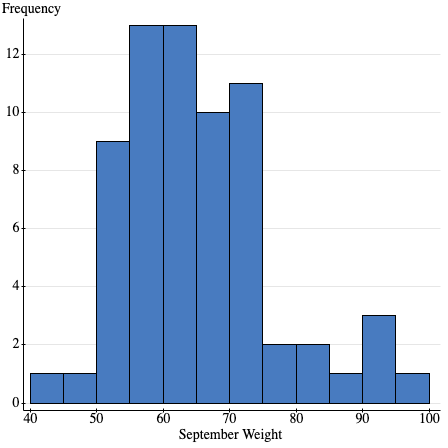
\includegraphics[width=8cm]{assets/september-weights.png}
  \caption{September Weights}
\end{figure}

\pagebreak
\subsection{Appropriate Measure of Central Tendency}
In this case I believe the \textbf{mean} would be the most appropriate measure of central tendency. There don't appear to be any outliers or values that would strongly skew the value of the mean.

\subsection{Relationship Between September Weights \& BMI}
There appears to be a relationship between the differences in September weights and BMI, although it is definitely not 1:1. In general, as indicated by the Index/Time Plot, their respective values tended to be proportional.
\begin{figure}[ht]
  \centering
  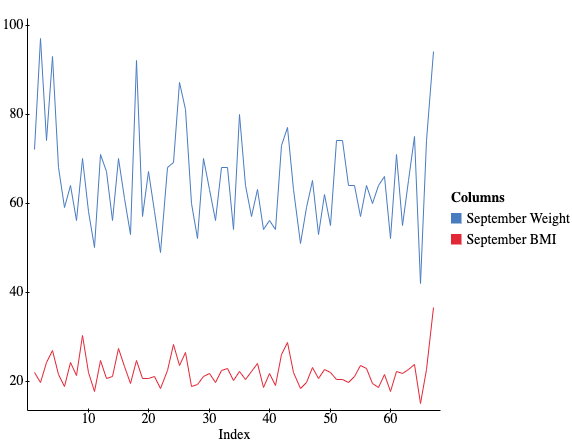
\includegraphics[width=8cm]{assets/weights-and-bmi.png}
  \caption{Weights \& BMI}
\end{figure}

\pagebreak
\subsection{September BMI for Males \& Females}
Overall it appears that the males surveyed had higher BMI values than the females. All five numbers from the five number summary register higher for males.
\begin{figure}[ht]
  \centering
  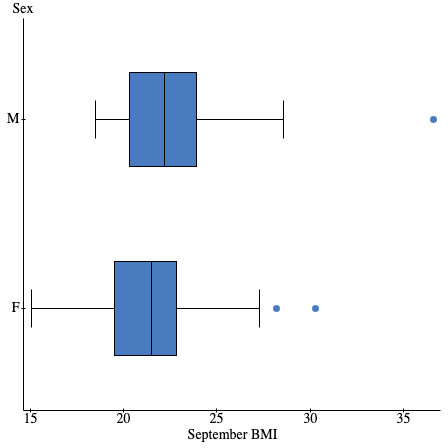
\includegraphics[width=8cm]{assets/males-vs-females.png}
  \caption{Weights \& BMI}
\end{figure}


\end{document}
